\documentclass{article}
\usepackage{graphicx}
\usepackage{pgfplots}
\pgfplotsset{compat=1.18}
\usetikzlibrary{positioning,arrows.meta}
\graphicspath{{figures/}}

\begin{document}

\section{TikZ in the editor}
The editor has no TeX engine, so it does not draw TikZ. A picture written in the document shows as code in the visual view and as a card in the preview, and still compiles as usual:

\begin{figure}[h]
  \centering
  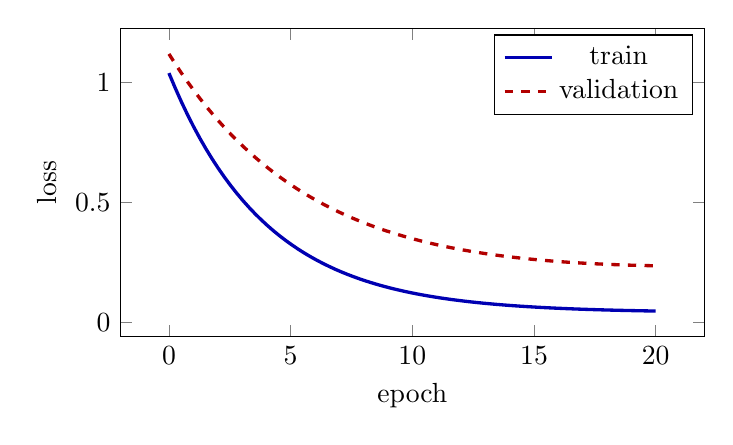
\begin{tikzpicture}
    \begin{axis}[width=9cm, height=5.5cm, xlabel={epoch}, ylabel={loss}]
      \addplot[blue!70!black, very thick, domain=0:20, samples=80] {exp(-x/4) + 0.04};
      \addplot[red!70!black, very thick, dashed, domain=0:20, samples=80] {exp(-x/6) + 0.12 + 0.004*x};
      \legend{train, validation}
    \end{axis}
  \end{tikzpicture}
  \caption{A pgfplots plot, written in place.}\label{fig:inplace}
\end{figure}

\section{Compiled pictures}
Compiled on its own (\verb|figures/loss.tex| with pdflatex, then made a PNG) and included as an image, the same plot is drawn. Compile it again and the editor shows the new version within a few seconds.

\begin{figure}[h]
  \centering
  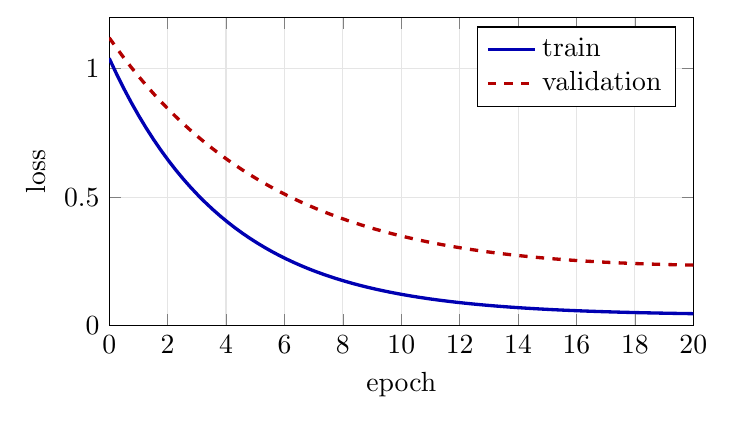
\includegraphics[width=0.75\linewidth]{loss}
  \caption{The plot of Figure~\ref{fig:inplace}, compiled.}\label{fig:loss}
\end{figure}

\begin{figure}[h]
  \centering
  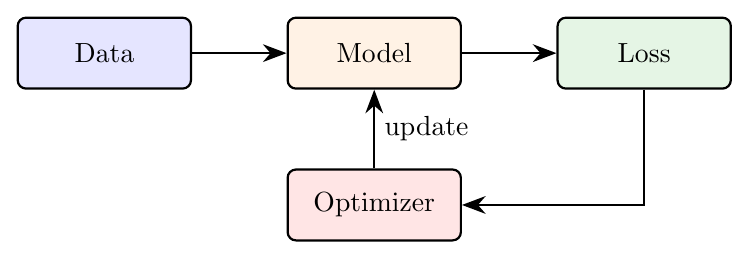
\includegraphics[width=0.75\linewidth]{pipeline}
  \caption{A TikZ diagram, compiled from \texttt{figures/pipeline.tex}.}\label{fig:pipeline}
\end{figure}

Figures~\ref{fig:loss} and~\ref{fig:pipeline} come from \verb|figures/*.tex|.
\end{document}
